\chapter{Control Schemes}
\textit{The satellite control schemes are introduced starting from the top of the hierarchy. The chosen reaction wheel desaturation control scheme determines the overall control structure, while allowing modification of other control blocks, making the system modular. Three different main attitude controllers are discussed}

\sout{In this chapter the purpose is to describe the design of the controllers for the satellite. First, a desaturation controller is designed for distributing the torque between the actuators. A second controller is the hybrid attitude one, which is capable of taking care of the tumble of the satellite. Next, based on previous work, two types of attitude controllers are designed. For making a comparison between a linear controller and non-linear one, a state feedback controller and a sliding mode controller are presented.}


\todo{evaluation of station tracking precision - should be within $1\deg$. Compare different reaction wheel configurations}

When developing complex systems, using a modular design, setting up a hierarchy between elements, and using abstractions can be very helpful in keeping the complexity at a manageable level. They can also prove to be useful during debugging or finding faults in the system. The proposed control scheme utilizes these tools. Figure  \ref{fig:mainLoop} introduces the high-level control scheme used in the thesis. The scheme is inspired by the control scheme proposed by Trégouët et al. in their paper concerning a new desaturation control scheme \cite{DesatTregouet}. 

%The proposed high-level control scheme presented in figure \ref{fig:mainLoop} has a hierarchical, modular structure.
 The main attitude controller outputs a torque reference for the actuators, which is then distributed by lower level controllers. This means that the attitude controller can be swapped without having to modify the lower level controllers. The desaturation controller distributes the torque between the reaction wheels and magnetorquers. The reaction wheel subsystem executes local fault detection and fault isolation. It receives a 3 dimensional torque demand and distributes it between the individual reaction wheel motors. The reaction wheel subsystem checks fault residual signals and adjusts torque distribution between reaction wheels accordingly. These will be elaborated in subsequent sections.
 
\begin{figure}[h!]
	\centering 
	\includegraphics[width=160mm]{figures/mainLoop.pdf}	
	\caption{Main Control Loop.}
	\label{fig:mainLoop}
\end{figure}

The attitude dynamics are given once again by equation \ref{eq:sysDynMain}. 

\begin{equation}
\underline{I}_{s}\vec{\dot{\omega}} + \underline{\omega}^\times\underline{I}_{s}\vec{\omega} = -\vec{\dot{h}}_{rw} -  \underline{\omega}^\times \vec{{h}}_{rw} + \vec{N_{mt}}  + \vec{N_{dist}} =  -  \underline{\omega}^\times \vec{{h}}_{rw} + \vec{N_{rw}} + \vec{N_{mt}}  + \vec{N_{dist}}
\label{eq:sysDynMain} 
\end{equation}

The system's mechanical states affecting the attitude dynamics include satellite attitude, satellite angular velocity and reaction wheel angular velocity. High reaction wheel angular momenta can make the satellite react differently to the same control torques compared to when the reaction wheels are not rotating (e.g. smaller angular acceleration). Desaturation is reducing this unwanted effect, but it works quite slowly, requiring several orbits to reduce wheel angular velocity to an acceptable level. To counteract the unwanted gyroscopic term $\underline{\omega}^\times \vec{{h}}_{rw}$, the torque demand should include a compensation term for it.



\section{Desaturation}

The reaction wheel DC motors and bearings have a limited angular velocity range they can operate in. When the velocity reaches the limit, the motor can no longer accelerate the wheel further in one of the two directions, thus reducing controllability. To avoid this, the wheel velocity should be kept near a small reference angular velocity. Usually the speed is above zero to avoid static friction in the bearings. Decreasing the reaction wheel speed by transferring its angular momentum is called desaturation. Desaturation also decreases the the reaction wheels' gyroscopic term's effect on the overall satellite dynamics.

Reaction wheels are used to control the attitude of the satellite by controlling its angular momentum. This is done by transferring angular momentum between the reaction wheels and the satellite body. This leaves the sum of the satellite body's and wheels' angular momentum unchanged. When transferring the angular momentum from the reaction wheels back to the satellite body is not aligned with the control goal, angular momentum should be discarded in a different way. Magnetorquers are capable of desaturation since they can interact with the Earth's magnetic field and are able to transfer angular momentum of the satellite body to earth. Since the Earth's magnetic field is quite weak, the torque produced by magnetorquers are small compared to the torque of the reaction wheels. A further drawback of magnetorquers is that even if they are set up in an orthogonal configuration, they can only assert torques in a 2 dimensional plane at any given moment, the plane perpendicular to Earth's magnetic field. Reaction wheels can be used for fast attitude control while magnetorquers are good for gradually desaturating the reaction wheels over several orbits.

The angular momentum transfer happens through the satellite's body, but with the right control scheme. the desaturation can be  completely decoupled from attitude control. Trégouët et al. \cite{DesatTregouet} developed a cascaded control method for reaction wheel desaturation. The method is a revised version of the so-called cross-product control law. 
%
%
%The attitude dynamics are given once again by equation \ref{eq:sysDynMain}. 
%
%\begin{equation}
%\underline{I}_{s}\vec{\dot{\omega}} + \underline{\omega}^\times\underline{I}_{s}\vec{\omega} = -\vec{\dot{h}}_{rw} -  \underline{\omega}^\times \vec{{h}}_{rw} + \vec{N_{mt}}  + \vec{N_{dist}} =  -  \underline{\omega}^\times \vec{{h}}_{rw} + \vec{N_{rw}} + \vec{N_{mt}}  + \vec{N_{dist}}
%\label{eq:sysDynMain} 
%\end{equation}
%
%The system's mechanical states affecting the attitude dynamics include satellite attitude, satellite angular velocity and reaction wheel angular velocity. High reaction wheel angular momenta can make the satellite react differently to the same control torques compared to when the reaction wheels are not rotating (e.g. smaller angular acceleration). Desaturation is reducing this unwanted effect, but it works quite slowly, requiring several orbits to reduce wheel angular velocity to an acceptable level. To counteract the unwanted gyroscopic term $\underline{\omega}^\times \vec{{h}}_{rw}$, the torque demand should include a compensation term for it.


\subsubsection{Classical Cross Product Control Law}

The cross product control law achieves desaturation by using two control loops that are designed separately. The \textbf{attitude control loop} treats the reaction wheel torque as control input, the magnetorquer torque as disturbance, according to equation \ref{eq:desatDynClassic}.

\begin{equation}
\underline I_{s} \vec{\dot{\omega}} + \underline{\omega}^\times(\underline I_{s} \vec{\omega} + \vec{h_{rw}})  =    \overbrace{ \vec{N_{rw}}}^{\vec{u}} +  \overbrace{\vec{N_{mt}}}^{\vec{d}}
\label{eq:desatDynClassic}
\end{equation}

%When applying reaction wheel gyroscopic term compensation, the control law changes to what is shown in equation \ref{eq:desatDynReorder}.


%By rearranging equation \ref{eq:sysDynMain}, the satellite dynamics can be expressed according to equation \ref{eq:desatDyn}.
%\begin{equation}
%\underline I_{s} \vec{\dot{\omega}} + \underline{\omega}^\times(\underline I_{s} \vec{\omega} + \vec{h_{rw}}) = \vec{N_{rw}} +  \vec{N_{mt}} + \vec{N_{dist}} = \vec{N_{ctrl}} + \vec{N_{dist}}
%\label{eq:desatDyn}
%\end{equation}

If the control goal is to rotate the satellite, it might be desired to make the apparent satellite dynamics independent of reaction wheel angular momenta. This can be achieved by using the actuators to counteract the effect of the gyroscopic term $\underline{\omega}^\times \vec{h_{rw}}$. This is a form of state compensation. Equation \ref{eq:desatDynReorder} presents the attitude control loop terms corresponding to $\vec{u}$ control input and to $\vec{d}$ disturbance. $\vec{N_{dist}}$ is discarded from the discussion of the desaturation scheme.
\nomenclature[Su]{$\vec{u}$}{Control input}
\nomenclature[Sd]{$\vec{d}$}{Disturbance input}

\begin{equation}
\underline I_{s} \vec{\dot{\omega}} + \underline{\omega}^\times\underline I_{s} \vec{\omega} =    \overbrace{-\underline{\omega}^\times\vec{h_{rw}} + \vec{N_{rw}}}^{\vec{u}} +  \overbrace{\vec{N_{mt}}}^{\vec{d}}
\label{eq:desatDynReorder}
\end{equation}

Equation \ref{eq:desatDynReorder} implies that the task state compensation is assigned to the reaction wheels according to \ref{eq:stateComp}.

\begin{equation}
\vec{N_{rw}} = -\vec{\dot{h}_{rw}} = \vec{u} +  \underline{\omega}^\times\vec{h_{rw}}
\label{eq:stateComp}
\end{equation}

%\begin{align*}
%	\begin{split}
%		{\vec{\dot{\omega}}} &={-\underline I_{s}^{-1}\underline S(\vec \omega)\underline I_{s}\vec \omega-\underline I_{s}^{-1}\underline S(\vec \omega)\vec h_{rw}-\underline I_s ^{-1}\vec{  N_{rw}} + \underline I_s ^{-1}(\vec{  N_{mt}} + \vec{  N_{dist}})} = \\
%		&= {\underline I_{s}^{-1}} [\vec{  N_{dist}} + \vec{  N_{ctrl}} - S(\vec \omega) (\underline I_{s}\vec \omega + \vec h_{rw})] 
%	\end{split}
%\end{align*}

The goal of the \textbf{momentum dumping loop} is to track the reference angular momenta of the reaction wheels. The dynamics of the momentum dumping loop is described by equation \ref{eq:momDumpDyn}. Introducing a constant angular velocity reference in the equation can be utilized to design a reference tracking control law subsequently.

\begin{equation}
\label{eq:momDumpDyn}
\dot{\vec{h_{rw}}} = \frac{d}{dt}(\vec{h_{rw}} - \vec{h_{ref}}) = -\underline{B}^\times(t) \vec{m_{mt}} 
\end{equation}
where $\vec{m_{mt}}$ is the magnetic moment of the magnetorquers, $\vec{B}$ is the local geomagnetic field in SBRF, $\vec{h_{rw}}$ is the angular momentum vector of the reaction wheels, $\vec{h_{ref}}$ is the reference reaction wheel angular momentum for desaturation.

%\begin{equation}
%\label{eq:momDumpDyn}
%\frac{d\vec{h_{rw}}}{dt} = \frac{d}{dt}(\vec{h_{rw}} - \vec{h_{ref}}) = -\underline{B}^\times(t) \vec{m_{mt}} =  \frac{\underline{B}^\times(t) \underline{B}^\times(t)}{|\vec{B}(t) |^2} k_p\left(\vec{h_{rw}} - \vec{h_{ref}} \right)
%\end{equation}

Using the dynamics in equation \ref{eq:momDumpDyn}, the momentum dumping control law can be designed to stabilize around $\vec{h_{ref}}$. The original cross product control does exactly that.
The cross-product control law controls the magnetorquers' magnetic momentum using a negative feedback on the difference between the angular momentum of the reaction wheels and their reference angular momentum, as shown in equation \ref{eq:crossLaw}.

\begin{equation}
\label{eq:crossLaw}
\vec{m_{mt}} = -\frac{\underline{B}^\times(t)}{|\vec{B}(t) |^2} k_p\left(\vec{h_{rw}} - \vec{h_{ref}} \right)
\end{equation}
where $k_p$ is an adjustable proportional gain.

		\nomenclature[Sm]{$\vec{m_{mt}}$}{Magnetorquer magnetic moment}
		\nomenclature[SB]{$\vec{B}$}{local geomagnetic field in body fixed frame}
		\nomenclature[Sh]{$\vec{h_{rw}}$}{The angular momentum vector of the reaction wheels}
		\nomenclature[Sh]{$\vec{h_{ref}}$}{The reference angular momentum vector of the reaction wheels}
		\nomenclature[Sh]{$\vec{h_{T}}$}{Total angular momentum of the satellite}	
		
Recognizing that the reaction wheels cannot change $\vec{h_{T}}^{[I]}$ total angular momentum, a step can be taken towards detaching the effect of the magnetorquers and the reaction wheels. Substituting $ \vec{h_{rw}} = \underline{R}(^s_i\vec{ q}) \vec{h_{T}^{[I]}} - \underline{I}_s \vec{\omega}$. Using this, equation \ref{eq:crossLaw} can be rewritten according to equation \ref{eq:bodyDesatRewrite}.

\begin{align}
\vec{m_{mt}} = 
-  \frac{\underline{B}^{\times}(t)}{|\vec{B}(t) |^2} k_p\left(\underline{R}(^s_i\vec{ q}) \vec{h_{T}^{[I]}} -  \underline{I}_s \vec{\omega} - \vec{h_{ref}}\right) 
%-  \frac{(\underline{R}(^s_i\vec{ q}) \underline{B}^{[I]}(t))^\times}{|\vec{B}(t) |^2} k_p\left(\underline{R}(^s_i\vec{ q}) \vec{h_{T}^{[I]}} -  \underline{I}_s \vec{\omega} - \vec{h_{ref}}\right) 
%= 
%-\underline{R}(^s_i\vec{ q})  \frac{\underline{B}^{[I]\times}(t)}{|\vec{B^{[I]}}(t) |^2} k_p\left(\vec{h_{T}^{[I]}} - \vec{h_{ref}} + \underline{R}^T(^s_i\vec{ q}) \overbrace{
%	\left( \left( \underline{R}(^s_i\vec{ q}) - \underline{1}_3 \right) \vec{h_{ref}} - \underline{I}_s\vec{\omega} \right)}^{\xi(\vec{q}, \vec{\omega})} \right)\\
%= -\underline{R}(^s_i\vec{ q})  \frac{\underline{B}^{[I]\times}(t)}{|\vec{B^{[I]}}(t) |^2} k_p\left(\vec{h_{T}^{[I]}} - \vec{h_{ref}} + \underline{R}^T(^s_i\vec{ q}) \vec{\xi}(\vec{q}, \vec{\omega}) \right)
\label{eq:bodyDesatRewrite}
\end{align}		


			
Momentum dumping and attitude control can potentially be opposing goals, since attitude control changes the reaction wheel velocity to produce the required torque, while the desaturator tries to keep the angular velocity close to the reference. 
Further analysis made by Trégouët et al. \cite{DesatTregouet} found that the classical cross product control law can be interpreted as having a quasi-cascaded structure with the momentum dumping loop including the magnetorquers as the upper subsystem and the attitude control loop with the reaction wheels being the lower subsystem. The problem is that there's a feedback involved from the lower subsystem to the upper one, making $\frac{d}{dt}(\vec{h_{rw}} - \vec{h_{ref}})$ dependent on the attitude parameters, as shown in equation \ref{eq:momDumpDynDependency}.  

% In order to better distinguish the effect of the magnetorquers and reaction wheels, an inertial frame based expression of $\vec{h_T^{[I]}}$  is utilized. The reaction wheels can't change $\vec{h_T^{[I]}}$. $\xi(\vec{q}, \vec{\omega})$ denotes the momentum dumping loop's dependency on $\vec{q}$ and $\vec{\omega}$.
		
		\begin{figure}[h]
			\centering
			\begin{tabular}{@{}c@{\hspace{.5cm}}c@{}}
				\includegraphics[page=1,width=1\textwidth]{quasiCascadeDesat.pdf}
			\end{tabular}
			\caption{Quasi cascaded desaturation control scheme \cite[Fig. 2.]{DesatTregouet}}
			\label{fig:quasiCascadeDesat}
		\end{figure}
	
		
\begin{align}
\nonumber \vec{m_{mt}} = 
- \frac{(\underline{R}(^s_i\vec{ q}) \underline{B}^{[I]}(t))^\times}{|\vec{B}(t) |^2} k_p\left(\underline{R}(^s_i\vec{ q}) \vec{h_{T}^{[I]}} -  \underline{I}_s \vec{\omega} - \vec{h_{ref}}\right)  \\
\nonumber =
-\underline{R}(^s_i\vec{ q})  \frac{\underline{B}^{[I]\times}(t)}{|\vec{B^{[I]}}(t) |^2} k_p\left(\vec{h_{T}^{[I]}} - \vec{h_{ref}} + \underline{R}^T(^s_i\vec{ q}) \overbrace{
	\left( \left( \underline{R}(^s_i\vec{ q}) - \underline{1}_3 \right) \vec{h_{ref}} - \underline{I}_s\vec{\omega} \right)}^{\xi(\vec{q}, \vec{\omega})} \right)\\
= -\underline{R}(^s_i\vec{ q})  \frac{\underline{B}^{[I]\times}(t)}{|\vec{B^{[I]}}(t) |^2} k_p\left(\vec{h_{T}^{[I]}} - \vec{h_{ref}} + \underline{R}^T(^s_i\vec{ q}) \vec{\xi}(\vec{q}, \vec{\omega}) \right)
\label{eq:momDumpDynDependency}
\end{align}		

where $\underline{1}_3$ is a $3\times3$ identity matrix, $\vec{\xi}(\vec{q}, \vec{\omega})$ is the notation for the term related satellite dynamics states that affect the desaturation dynamics.

Remapping equation \ref{eq:momDumpDynDependency} to inertial frame results in equation  \ref{eq:momDumpDynDependencyInertial}. Figure \ref{fig:quasiCascadeDesat} illustrates the system according to equations \ref{eq:desatDynReorder} and \ref{eq:momDumpDynDependencyInertial}.

\begin{equation}
\label{eq:momDumpDynDependencyInertial}
\vec{m_{mt}^{[I]}} = -\frac{\underline{B}^{[I]\times}(t)}{|\vec{B^{[I]}}(t) |^2} k_p 
\left(\vec{h_{T}^{[I]}} - \vec{h_{ref}} + \underline{R}^T(^s_i\vec{ q}) \xi(\vec{q}, \vec{\omega}) \right) 
	\end{equation}			

\subsubsection{Revised cross product control law}

In cascaded structure, the upper subsystem can undesirably disturb the lower one.
Since attitude control is more crucial than desaturation, it would be more desirable to use the attitude control loop as the upper subsystem and the momentum dumping loop as the lower one, as opposed to the reverse. This arrangement can be obtained by applying input allocation, i.e. 'suitably assigning the low level actuators' input, based on a higher level control effort requested by the control system' \cite{JOHANSEN20131087}. From the point of view of the desaturation controller, the control goal is to keep the reaction wheels' angular momentum as close to the reference momentum as possible. By using a modified version of the cross product control law, the desaturation controller dynamics can be decoupled from the attitude control loop, this way the desaturator can achieve its  control goal independently from the attitude control law. The control scheme is presented in Figure \ref{fig:CascadeDesat}.

		\begin{figure}[h]
			\centering
			\label{fig:decoupledDesat}
			\begin{tabular}{@{}c@{\hspace{.5cm}}c@{}}
				\includegraphics[page=1,width=1\textwidth]{cascadeDesat.pdf}
			\end{tabular}
			\caption{Cascaded desaturation control scheme  \cite[Fig. 4.]{DesatTregouet}}
			\label{fig:CascadeDesat}
		\end{figure}

%		\begin{equation}
%		\label{eq:modCrossControl}
%		\vec{\tau_{mt}}^{[I]} = -\frac{\underline{\tilde{b}}^{[I]\times(t)}}{|\vec{\tilde{b}^{[I]}}(t) |^2} k_p\left(\vec{h_{rw}}^{[I]} - \underline{R}^T(^i_s\vec{ q})\vec{h_{ref}} \right)
%		\end{equation}

The momentum dumping control law for the reverse cascade is derived in two steps. First, the control law for the original cascade scheme presented in \ref{eq:momDumpDynDependencyInertial} in ECI frame is revised to discard the feedback connection corresponding to $\vec{\xi}(\vec{q}, \vec{\omega})$, as presented in this subsection, second, input allocation is used to reverse the order of the cascade, as presented in the following section. The system can be turned into a cascade if the term $\vec{\xi}(\vec{q}, \vec{\omega})$ is eliminated from equation \ref{eq:momDumpDynDependencyInertial}.  The resulting control law is presented in equation \ref{eq:newMTcontrol}.

\begin{equation}
\label{eq:newMTcontrol}
\vec{m_{mt}^{[I]}} = -\frac{\underline{B}^{[I]\times}(t)}{|\vec{B^{[I]}}(t) |^2} k_p 
\left(\vec{h_{T}^{[I]}} - \underline{R}^T(^s_i\vec{ q})\vec{h_{ref}} \right) 
\end{equation}			

The dynamics of the total angular momentum and the satellite's angular velocity can be described according to equations \ref{eq:dyn01} and \ref{eq:dyn02}, where the total angular momentum dynamics is described in ECI frame, while the satellite angular velocity dynamics is described in SBRF frame. The magnetorquer torque is considered a disturbance, which is altering the total angular momentum of the system.

\begin{flalign}
\label{eq:dyn01}
\vec{\dot{h}_{T}}^{[I]} = -\underline{B}^{[I]}(t)^\times \vec{m_{mt}^{[I]}} \\
\label{eq:dyn02}
\underline I_{s} \vec{\dot{\omega}} + \underline{\omega}^\times\underline I_{s} \vec{\omega} =    \vec{u} + \underline{R}^T(^s_i\vec{ q}) \vec{\dot{h}_{T}}^{[I]}
\end{flalign}

%\underline I_{s} \vec{\dot{\omega}} + \underline{\omega}^\times\underline I_{s} \vec{\omega} =    \overbrace{-\underline{\omega}^\times\vec{h_{rw}} + \vec{N_{rw}}}^{\vec{u}} +  \overbrace{\vec{N_{mt}}}^{\vec{d}}

\subsubsection{Static allocation}

Equation \ref{eq:dyn02} suggests that the desaturation loop can have an effect on the on the attitude control loop, as mentioned above. That is undesired, since the attitude control loop is of higher importance than desaturation. To reverse the cascade arrangement corresponding to control law \ref{eq:newMTcontrol}, the grouping of the terms need to be revised first. For the reverse cascade scheme, the control input $\vec{u}$ is modified to include the magnetorquer torque, according to equation \ref{eq:newdesatDynReorder}. The magnetorquer torque is no longer handled as a disturbance, instead it is explicitly a term in the control input. If  $\vec{u}$ actuation tracking  $\vec{u}$ demand well, the main attitude dynamics becomes independent of the magnetorquer torque output.

\begin{equation}
\underline I_{s} \vec{\dot{\omega}} + \underline{\omega}^\times\underline I_{s} \vec{\omega} =    \overbrace{-\underline{\omega}^\times\vec{h_{rw}} + \vec{N_{rw}} +  \vec{N_{mt}}}^{\vec{u}}
\label{eq:newdesatDynReorder}
\end{equation}


With the new grouping, the reaction wheel torque reference can be expressed according to equation \ref{eq:newstateComp}. The equation suggests that if the in some cases the magnetorquers can 'help out' the reaction wheels, decreasing reaction wheel torque demand, thus decreasing reaction wheel acceleration. 

\begin{equation}
\vec{N_{rw}} =  \vec{u} - \vec{N_{mt}} +  \underline{\omega}^\times\vec{h_{rw}} 
\label{eq:newstateComp}
\end{equation}

%\begin{equation}
%\vec{N_{rw}} =  \vec{u} - \vec{N_{mt}} +  \underline{\omega}^\times\vec{h_{rw}} = 
%\vec{u} - \left( \underline{R}(\vec{ q})  \vec{B^{[I]}}(t)\right)^\times \vec{m_{mt}}  +  \underline{\omega}^\times\vec{h_{rw}} 
%\label{eq:newstateComp}
%\end{equation}


The momentum dumping dynamics becomes what is presented in SRBF by equation \ref{eq:newmomDumpDyn}, in ECI frame by equation \ref{eq:newmomDumpDyn2}. Transformation to inertial frame eliminates the gyroscopic term from the equation. Equation \ref{eq:newmomDumpDyn2} suggests that the desaturation dynamics is affected by the main attitude control input.

\begin{equation}
\label{eq:newmomDumpDyn}
\frac{d}{dt}(\vec{h_{rw}} - \vec{h_{ref}}) = -\vec{u} - \underline{\omega}^\times\vec{h_{rw}} - \left( \underline{R}(^s_i\vec{ q})  \vec{B^{[I]}}(t)\right)^\times \vec{m_{mt}}
\end{equation}

\begin{equation}
\label{eq:newmomDumpDyn2}
\vec{\dot{h}_{rw}^{[I]}} = -\underline{R}^T(^s_i\vec{ q})\vec{u}  - \vec{B^{[I]}}(t)^\times \vec{m_{mt}^{[I]}}
\end{equation}


%Equation \ref{eq:newmomDumpDynECI} describes the dynamics shown in equation \ref{eq:newmomDumpDyn} in ECI frame, the gyroscopic term disappears. It is apparent that the desaturation controller is affected by the attitude controller's $\vec{u}$ input, while the attitude controller is unaffected by the momentum dumping loop.
%
%\begin{equation}
%\label{eq:newmomDumpDynECI}
%\vec{\dot{h}_{rw}} = -\underline{R}^T(\vec{ q})\vec{u} -  \underline{B}^{[I]}(t)^\times \vec{m_{mt}^{[I]}}
%\end{equation}

The new magnetorquer magnetic moment control law is established for dynamics presented by equation \ref{eq:newmomDumpDyn2}, ignoring $\vec{u}$. The control law is given by equation \ref{eq:finalMTlawECI}. The control system consisting of equations \ref{eq:finalMTlawECI} and \ref{eq:newstateComp} are illustrated by figure \ref{fig:CascadeDesat}. Since the main attitude control loop is unaffected by the desaturation control loop, the main attitude controller can be considered as the upper subsystem of the cascade. The control law suggests that the sum of magnetorquer magnetic moments $\vec{m_{mt}^{[I]}} $ has no component in the direction of $\vec{B^{[I]}}$, since that would be a waste of energy.

\begin{equation}
\vec{m_{mt}^{[I]}} 
= - \frac{\underline{B}^{[I]}(t)^\times} {|\vec{B^{[I]}}(t) |^2} k_p\left(\vec{h_{rw}^{[I]}} - \underline{R}^T(^s_i\vec{ q})\vec{h_{ref}} \right)
\label{eq:finalMTlawECI}
\end{equation}


Figures \ref{fig:desatspeed} and \ref{fig:desatNmt} present desaturation over several orbits. The attitude controller control goal is nadir pointing, in the very beginning the attitude and angular velocity of the satellite differs from nadir pointing. The error is handled by quick reaction wheel torque action, then the wheels are desaturated over several orbits. The graphs show a semi-periodic magnetorquer behavior, corresponding to the periodic nature of Earth's magnetic field. By adjusting $k_p$ control gain in the magnetorquer control law, the speed of desaturation can be adjusted as well.


%\begin{equation}
%\vec{m_{mt}} 
%= - \frac{\left( \underline{R}(^s_i\vec{ q}) \underline{B}^{[I]}(t)\right)^\times} {|\vec{B^{[I]}}(t) |^2} k_p\left(\vec{h_{rw}} - \vec{h_{ref}} \right)
%\label{eq:finalMTlawBFF}
%\end{equation}

%The latter desaturation control structure can be viewed as if the amount of magnetorquer torque exerted is subtracted from the reaction wheel torque demand. When the torque demand is higher than the magnetorquer output torque, the magnetorquers help the reaction wheels, when it drops below a certain level, the magnetorquers are decreasing the angular momenta of the reaction wheels.

%\begin{equation}
%\label{eq:totalMomDyn}
%\vec{\dot{h}_T^{[I]}} = -\underline{B}^{[I]\times}(t) \vec{m_{mt}^{[I]}} 
%\end{equation}		
%
%\begin{equation}
%\underline I_{s} \vec{\dot{\omega}} + \underline{\omega}^\times\underline I_{s} \vec{\omega} =    
%\vec{u} +  \underline{R}^T(^i_s\vec{q})\vec{\dot{h}_T^{[I]}}
%\label{eq:newDesatDynInterpret}
%\end{equation}
		
%		where $\underline{R}(q)^T$ is the rotation matrix corresponding to rotation quaternion $^i_s\vec{ q}$ which transforms from body frame to inertial frame.
		

		
		
%		According to equation \todo{ref eq in modelling}
		

		%
		%\nomenclature[S]{$\underline{I}_{s}$}{Inertia matrix of the satellite}
		%\nomenclature[S]{$\vec{\omega}$}{Angular velocity of the satellite}
		%\nomenclature[S]{$\vec{N_{mt}$}{Magnetorquer torque}
		%	\nomenclature[S]{$\vec{N_{dist}$}{Disturbance torques}
		%		\nomenclature[S]{$\vec{u}$}{1}
		

		
		
%		\begin{equation}
%		\dot{x}_c = 0, (\vec{q},\vec{\omega},x_c) \in C\
%		\end{equation}
%		
%		\begin{equation}
%		x_c^+ = -x_c, (\vec{q},\vec{\omega},x_c) \in D\
%		\end{equation}
%		
%		\begin{equation}
%		\vec{u} = -c x_c \epsilon -K_\omega \vec{\omega}
%		\end{equation}
%		
%		\begin{equation}
%		C:= \left\lbrace (\vec{q},\vec{\omega},x_c) \in \mathbb{S}^3 \times \mathbb{R}^3 \times \left\lbrace -1,1 \right\rbrace : x_c\eta \geq -\delta \right\rbrace 
%		\end{equation}
%		
%		\begin{equation}
%		D:= \left\lbrace (\vec{q},\vec{\omega},x_c) \in \mathbb{S}^3 \times \mathbb{R}^3 \times \left\lbrace -1,1 \right\rbrace : x_c\eta \leq -\delta \right\rbrace 
%		\end{equation}
		
%		as shown in \ref{eq:finaleq}
%		\begin{flalign}
%		\vec{ ^s_i\dot q(t)}  = \dfrac{1}{2} \underline \Omega \  \vec{^s_i q(t)}
%		\end{flalign} 
		
		%\[
		%\begin{array}{l}
		%
		%\dot{x}_c = 0, (\vec{q},\vec{\omega},x_c) \in C\ \\ 
		%x_c^+ = -x_c, (\vec{q},\vec{\omega},x_c) \in D\ \\ 
		%\vec{u} = -c x_c \epsilon -K_\omega \vec{\omega} \\
		%C:= \left\lbrace (\vec{q},\vec{\omega},x_c) \in \mathbb{S}^3 \times \mathbb{R}^3 \times \left\lbrace -1,1 \right\rbrace : x_c\eta \geq -\delta \right\rbrace  \\
		%
		%D:= \left\lbrace (\vec{q},\vec{\omega},x_c) \in \mathbb{S}^3 \times \mathbb{R}^3 \times \left\lbrace -1,1 \right\rbrace : x_c\eta \leq -\delta \right\rbrace 
		%\end{array}
		%\]
		
%		\todo{this attitude controller should be down as one of the possible attitude controllers - "Satellite angular momentum removal utilizing the earth’s magnetic field" article}
		

		
		
		
%		\begin{equation}
%		\vec{\dot{\omega}} = \underline{I}_{s}^{-1}\left( \vec{u} -  \underline{\omega}^\times\underline{I}_{s}\vec{\omega}  \right) 
%		\end{equation}
		
%		\begin{equation}
%\vec{\tau_{mt}}^{[I]} = -\frac{\underline{\tilde{b}}^\times(t)}{|\vec{\tilde{b}}(t) |^2} k_p\left(\vec{h_{rw}}^{[I]} - \underline{R}^T(\vec{q})\vec{h_{ref}} \right)
%		\end{equation}

		
%\todo{apply to tetrahedron}
%\begin{figure}[h]
%	\centering
%	\begin{tabular}{@{}c@{\hspace{.5cm}}c@{}}
%		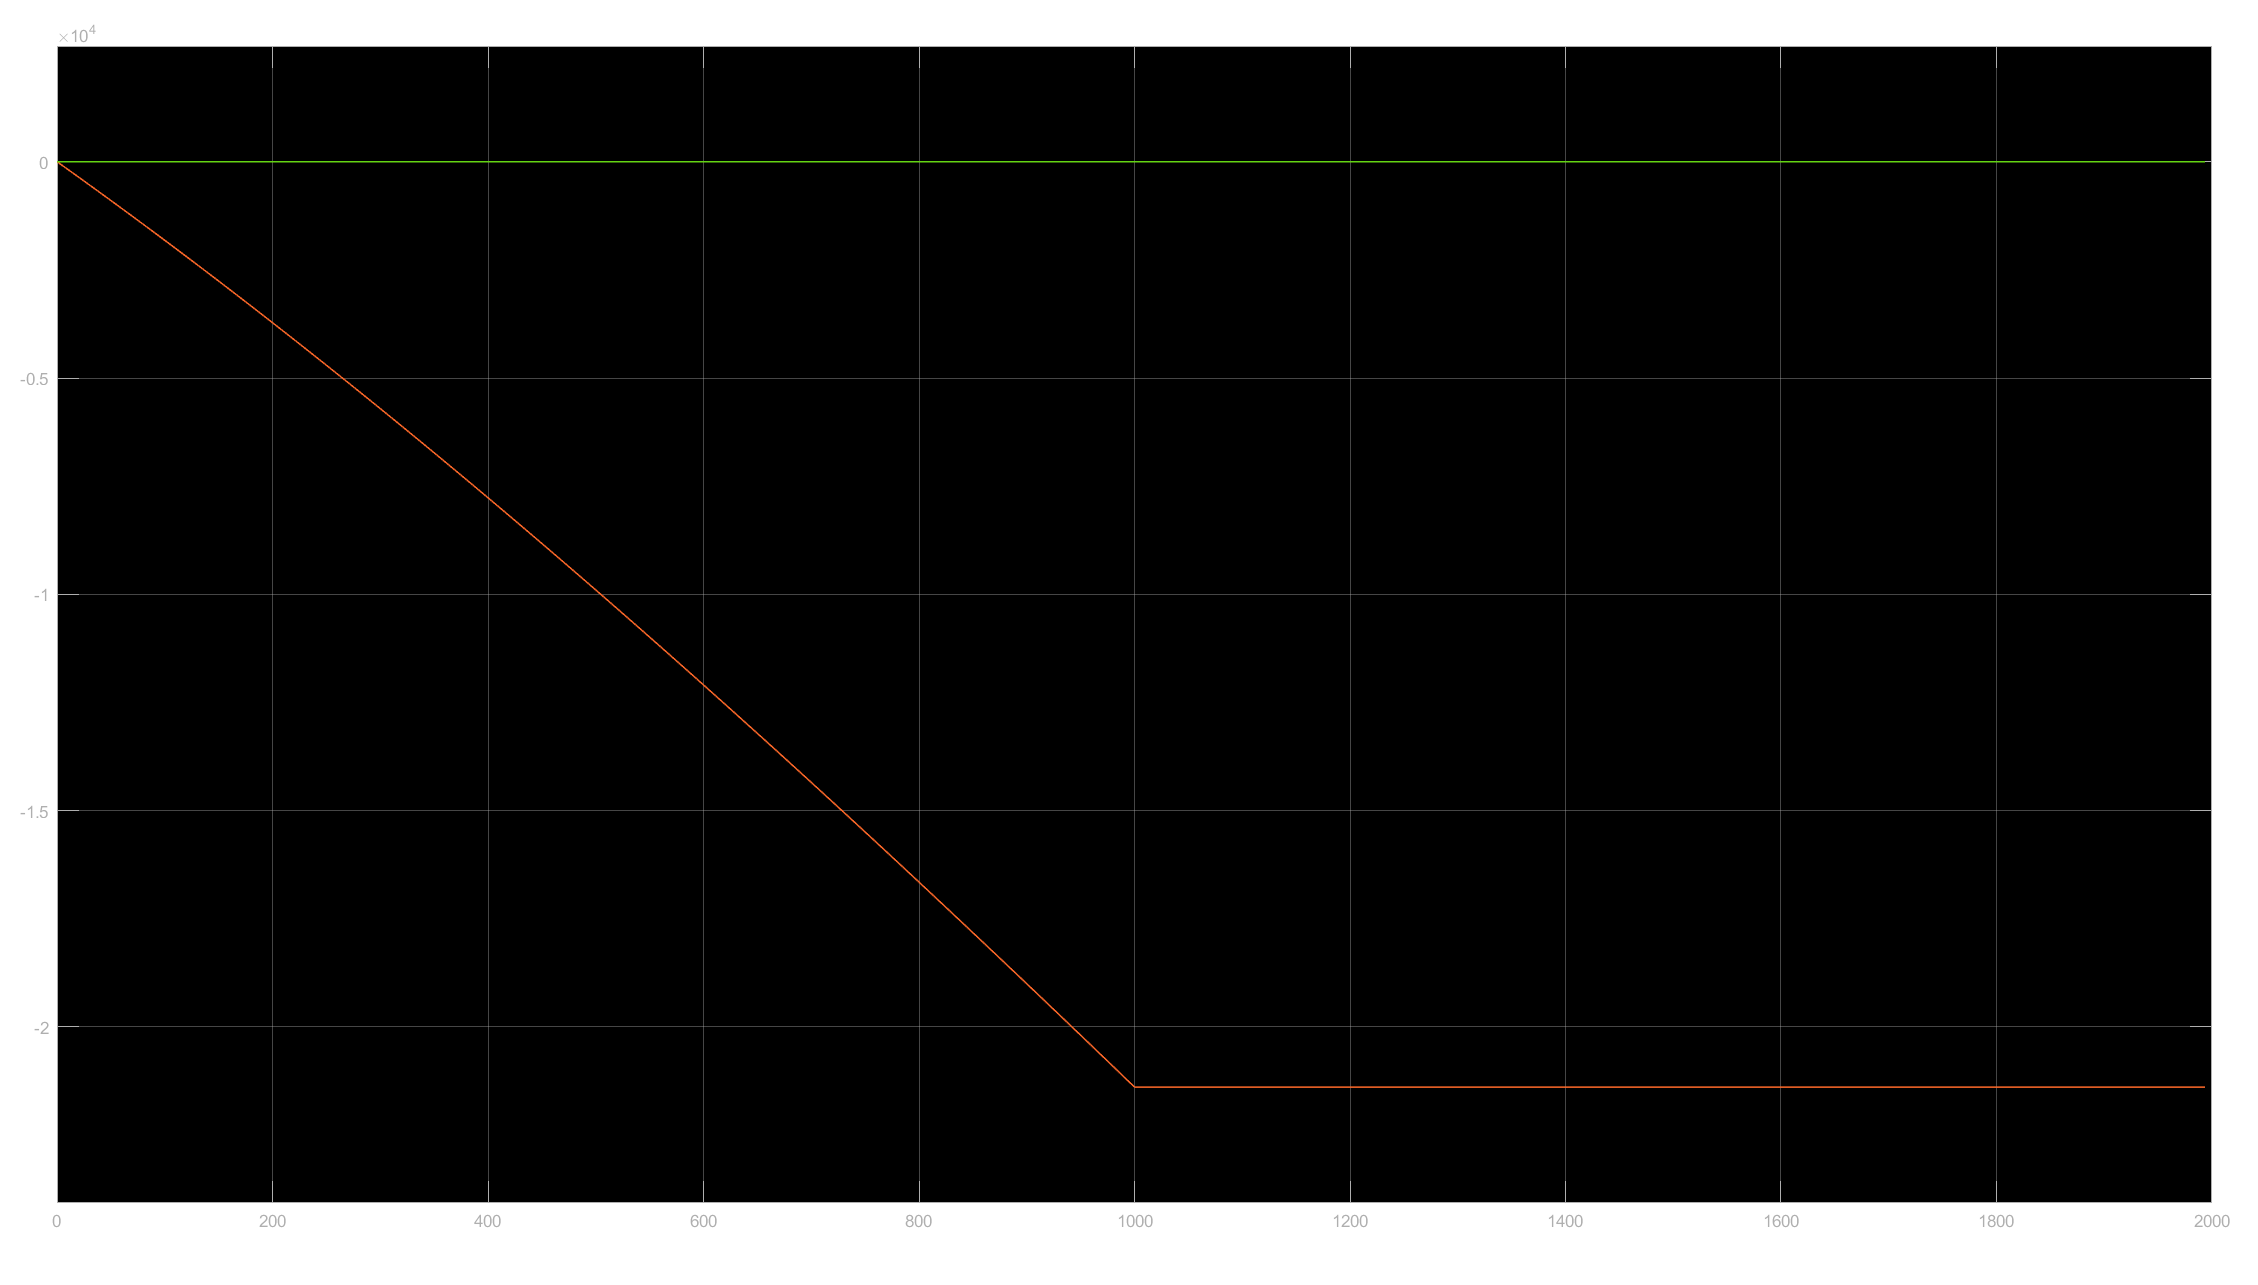
\includegraphics[page=1,width=1\textwidth]{noDesat3}
%	\end{tabular}
%	\caption{$\omega_rw$ Desaturation off, torque demand shut down at 1000 s}
%	\label{fig:DesatOff}
%\end{figure}
%
%\begin{figure}[h]
%	\centering
%	\begin{tabular}{@{}c@{\hspace{.5cm}}c@{}}
%		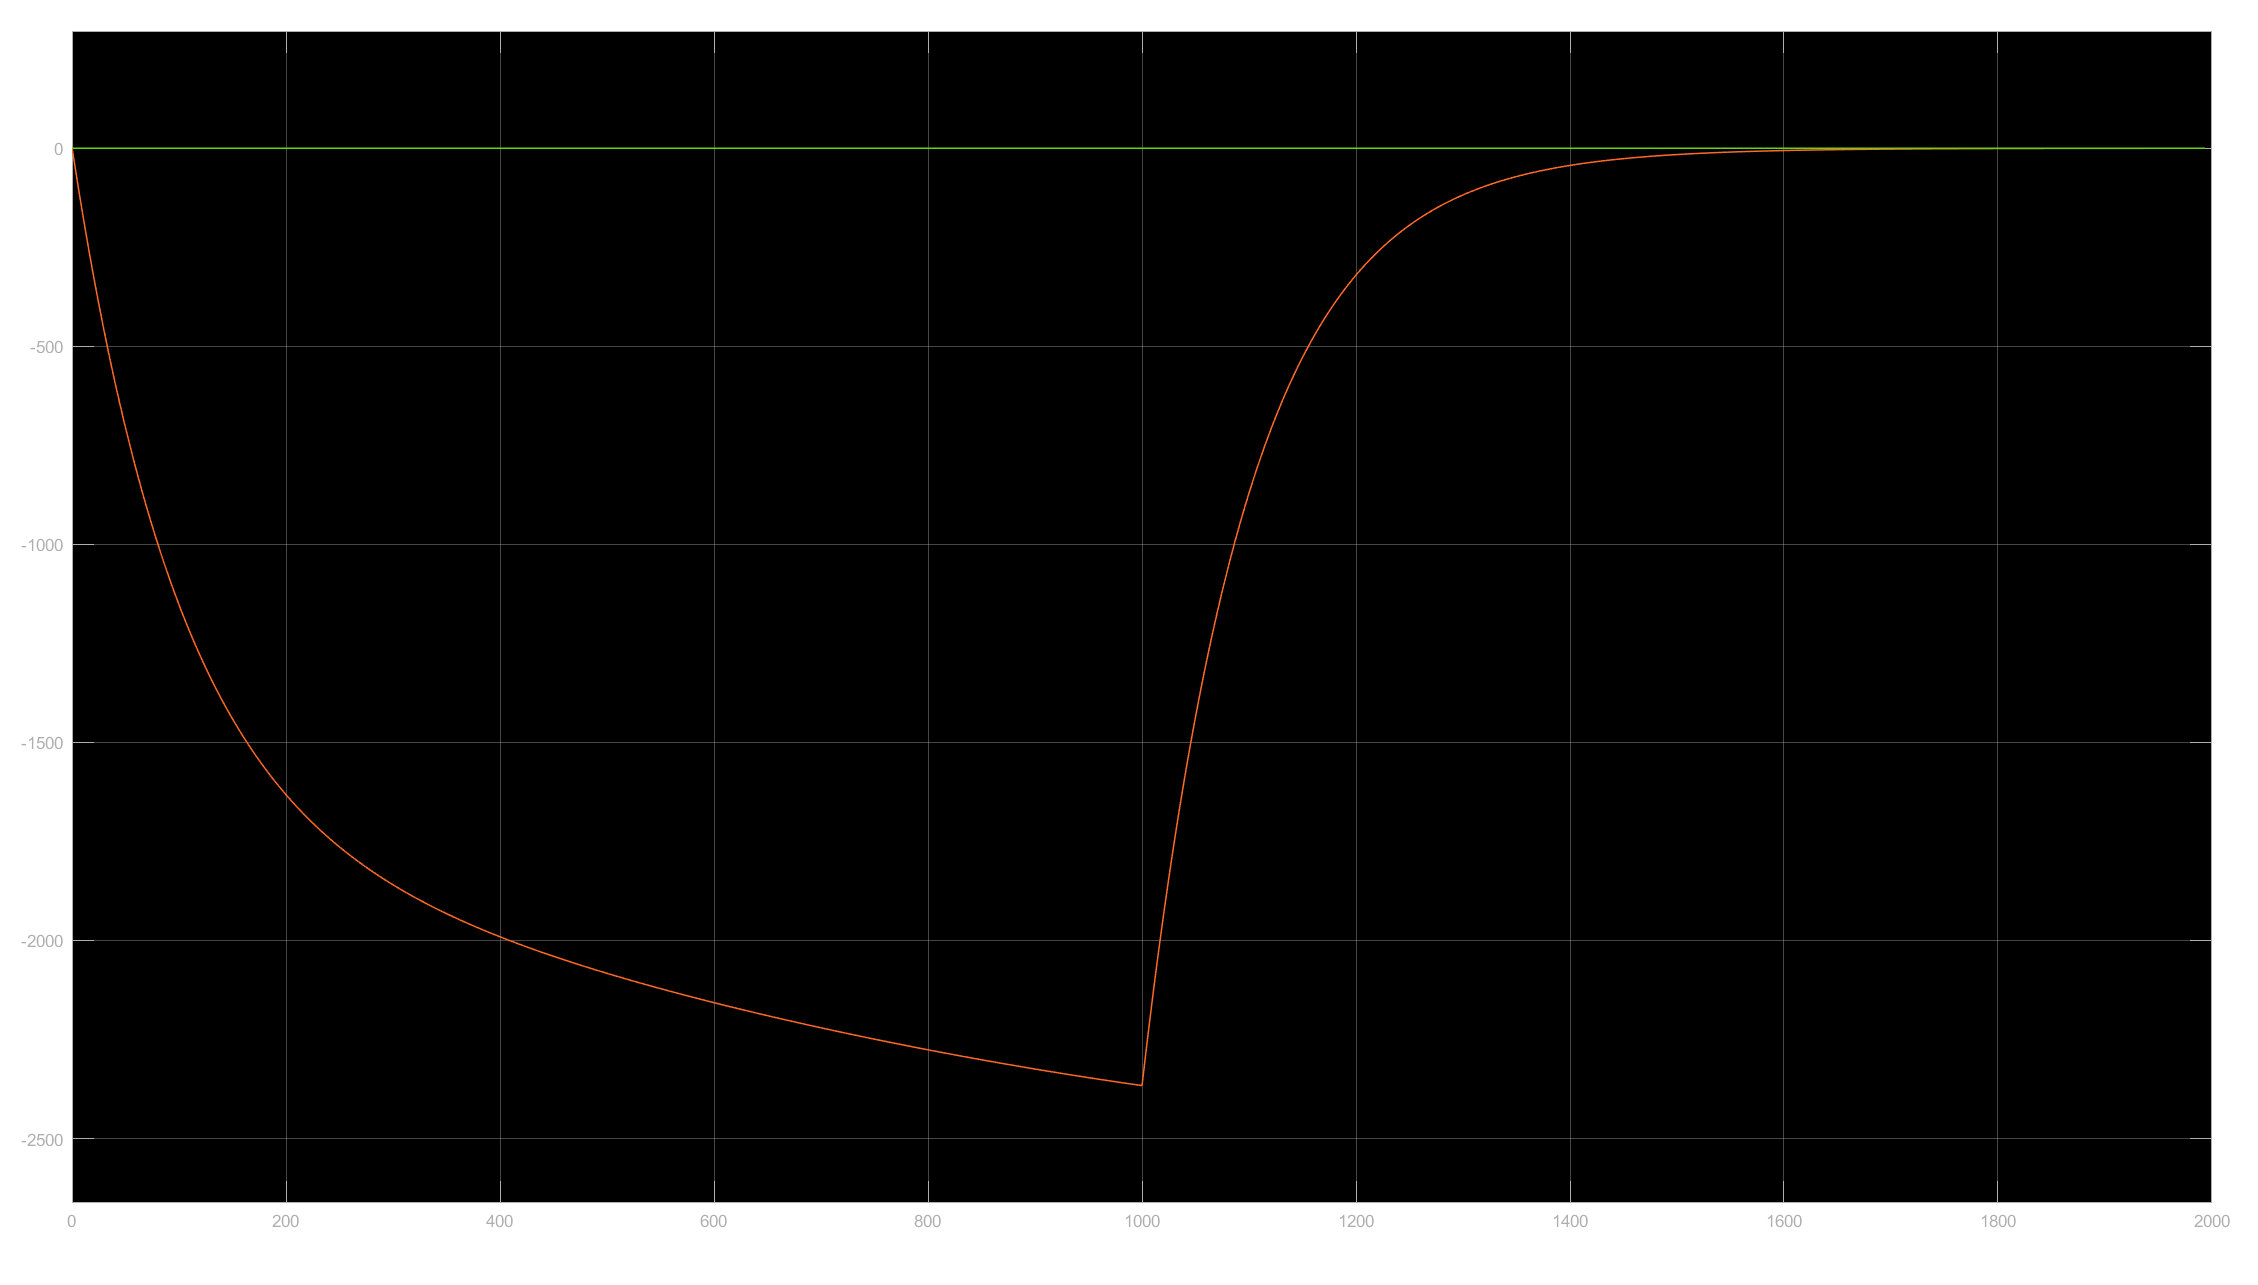
\includegraphics[page=1,width=1\textwidth]{desat3}
%	\end{tabular}
%	\caption{$\omega_rw$ Desaturation on}
%	\label{fig:DesatOn}
%\end{figure}

\begin{figure}[H]
	\centering
	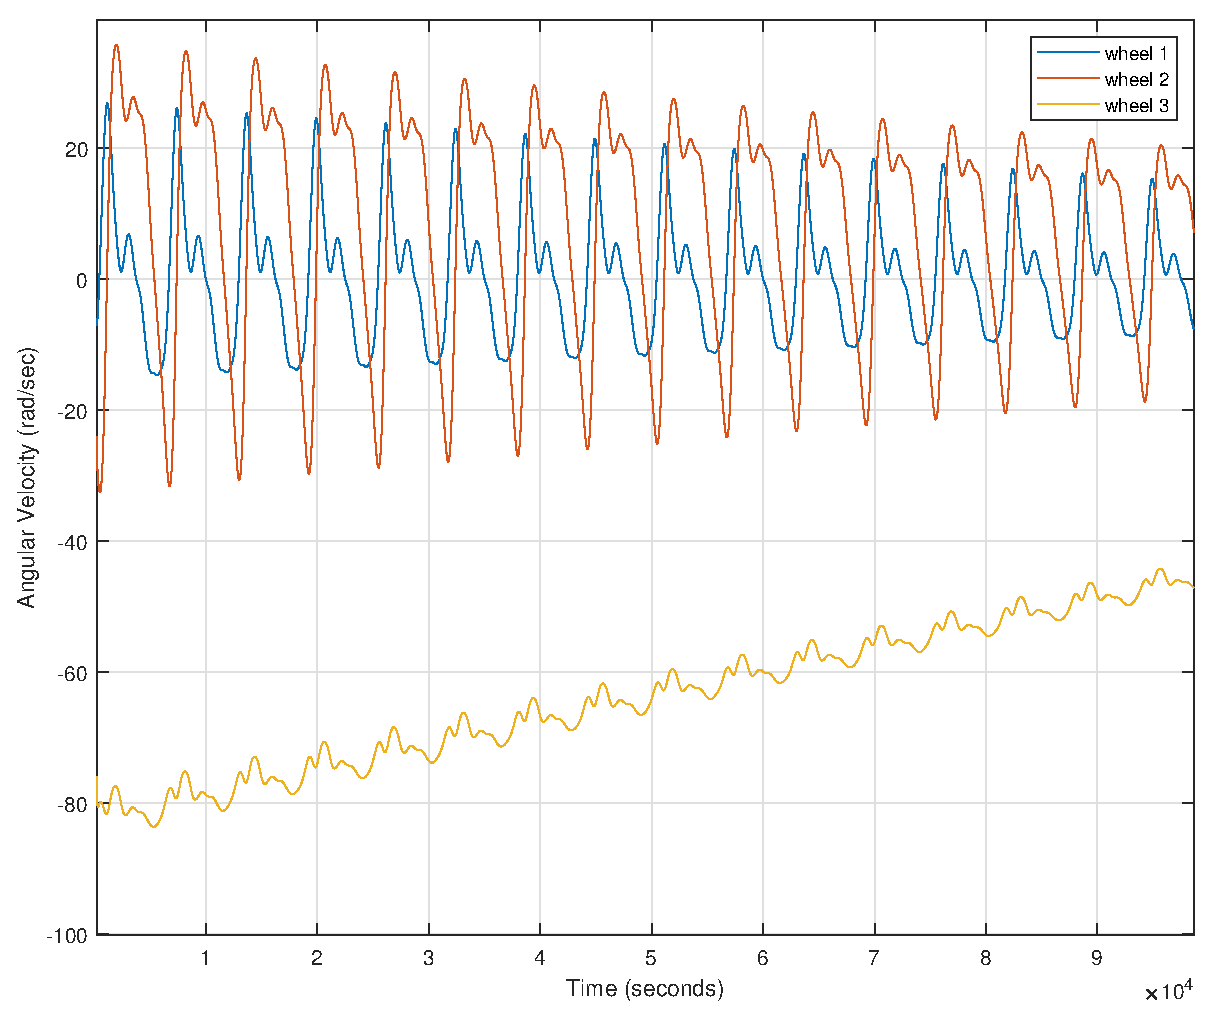
\includegraphics[width=0.7\linewidth]{figures/desaturation2}
	\caption{Angular velocity of reaction wheels in orthogonal configuration, during desaturation}
	\label{fig:desatspeed}
\end{figure}

\begin{figure}[H]
	\centering
	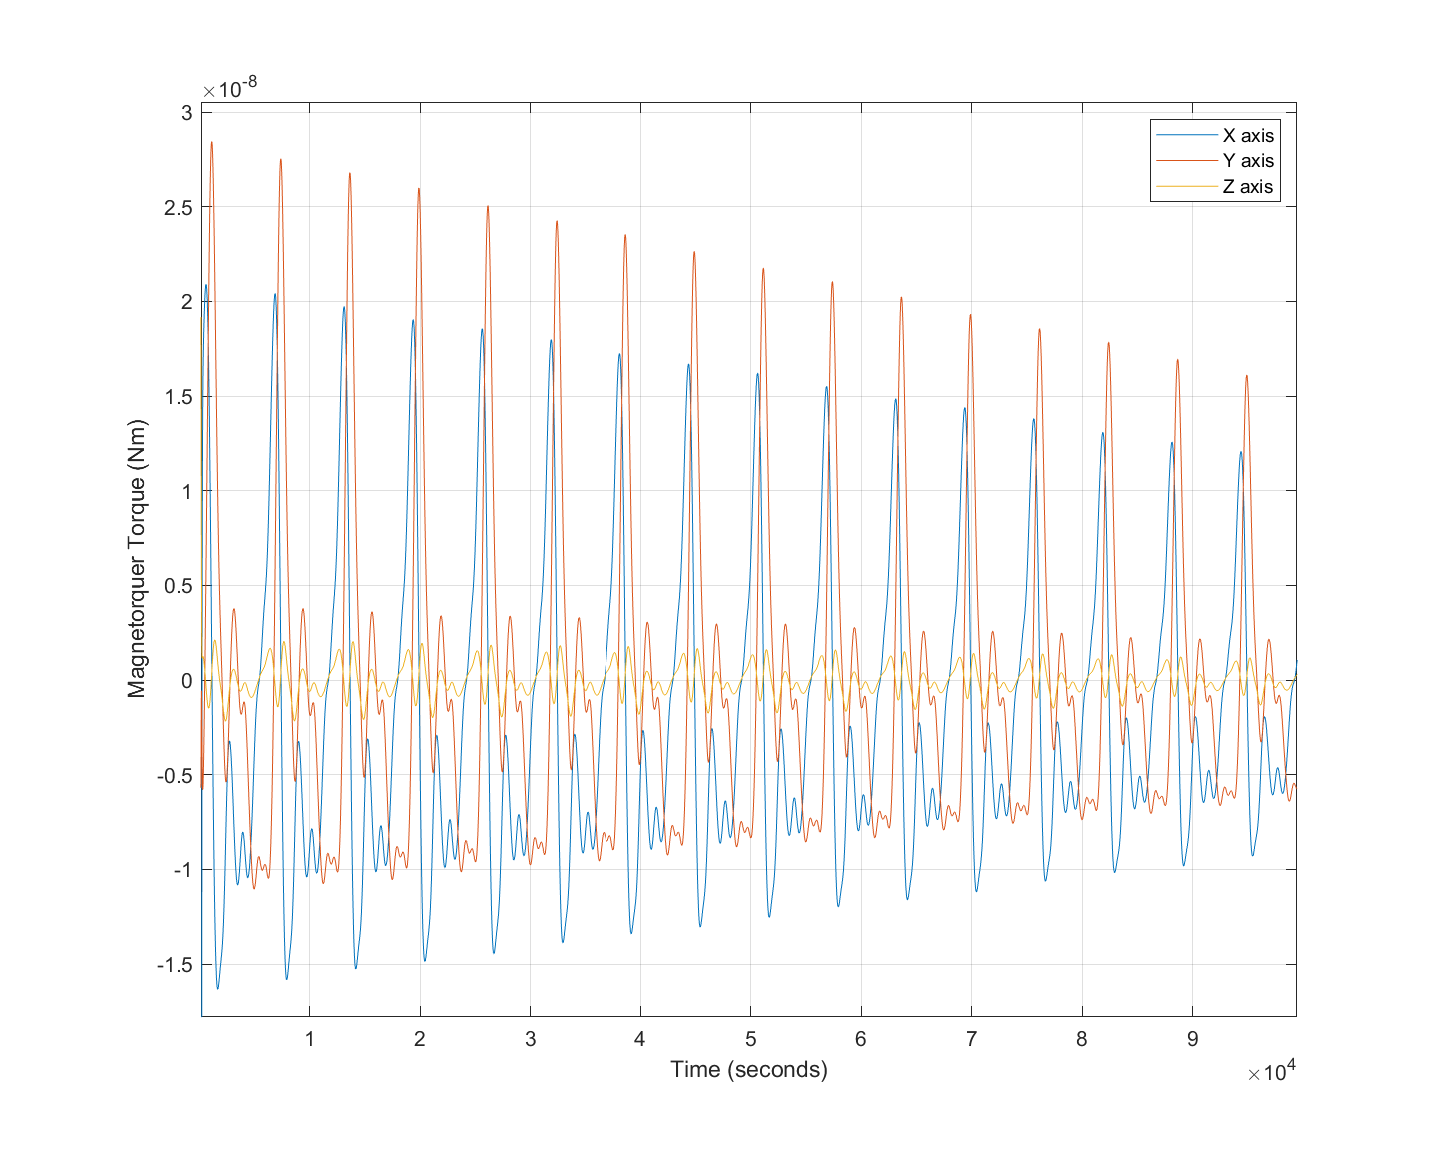
\includegraphics[width=0.8\linewidth]{figures/desat_Nmt}
	\caption{Magnetorquer torque $\vec{N_{mt}}$ during desaturation}
	\label{fig:desatNmt}
\end{figure}

\section{Hybrid Attitude Controller}

Dynamic discontinuous hybrid controller, global asymptotic stability, local exponential stability, state feedback for $\omega$ and $q$. Capable of detumbling. \cite{globalAttController}

One way of describing rotation in 3D Eucledian space is by using Euler sequences consisting of 3 rotational values. Euler rotation sequences can use combinations of roll, pitch and yaw. There's an inherent problem with Euler rotation, that makes controlling them an issue, i.e. they are disposed to singularities. Certain orientations might described by an infinite amount of different sequences. This situation can arise when the rotations are made in such a way that rotation axes align with each other. This issue is called the gimbal lock. The result is that given a attitude demand, the corresponding Euler rotations can not be unambiguously deducted, unless extra constraints are used.

Quaternion based rotation representation significantly improves control capabilities. Quaternions are not susceptible to singularities. The only problem with quaternion representation is the so-called double coverage, i.e. rotation by $-\vec{q}$ represents the same rotation as rotation by $-\vec{q}$. This becomes obvious from the rotation equation \ref{eq:doubleCover}.

\begin{equation}
\label{eq:doubleCover}
\vec{q} \vec{v} \vec{q}^{-1} = 	(\vec{-q}) \vec{v} (\vec{-q}^{-1})
\end{equation} 

The attitude control goal can be described as keeping the orientation demand $\vec{q}$. According to  \cite{globalAttController}, it is impossible to design a globally stabilizing quaternion based state feedback that is robust to measurement noise. The quaternion-based robust hysteric feedback controller which is capable of globally asymptotically stabilizing a rigid body is described subsequently. It can be considered as a more robust extension of classical state feedback controller.


The dynamics of a rigid body is described in equation \ref{eq:dynSimple}. For clarity of the control method, disturbance torques are emitted from the equation. For more details, refer to Appendix ... .

\begin{equation}
\label{eq:dynSimple}
\underline{I}_s \vec{\dot{\omega}} = \underline{\omega}^\times \underline{I}_s \vec{\omega} + \vec{N_{ctrl}}
\end{equation}

The control goal can be clearly described with rotation matrices. Rotation matrices use 9 variables to describe a rotation, but they have the advantage of being non-ambiguous. The rotation error can be described using equation \ref{eq:rotationError}. 

\begin{equation}
\label{eq:rotationError}
\underline{R}_e = \underline{R}(\vec{q_d})^T \underline{R}(\vec{q})
\end{equation}

The goal is to align the $\underline{R}(\vec{q})$ with $\underline{R}(\vec{q_d})$. If that demand is satisfied, $\underline{R}_e$ becomes $\underline{I}$ identity matrix. In quaternion representation, this goal corresponds to having having a unit quaternion with the scalar element being $\pm 1$, according to equation \ref{eq:stabilityQuat}. 

\begin{equation}
\label{eq:stabilityQuat}
\underline{R}_e = \underline{I} \xrightarrow{equivalent} \vec{q_e}  = \pm	\begin{bmatrix}
0 \\
0 \\
0 \\
1
\end{bmatrix} 	
\end{equation}

Because of the double coverage property of quaternions, stabilizing an attitude, stabilization has to be done on a two equilibrium points corresponding to $\vec{q_e}$ in equation \ref{eq:stabilityQuat}. According to \cite{globalAttController}, robust and global stabilization on this set is impossible to achieve using non-hybrid discontinuous state feedback in the presence of sensor noise. The paper proposes a hybrid, discontinuous, robust, gloablly asymptotically stabilizing attitude control method instead. A hybrid system is a system in which state changes can vary between being continuous or discrete.

The state changes are controlled by the following rules. Controller state storing information about which of the double covering quaternions should be tracked is introduced as $x_c \epsilon  \left\lbrace -1,1 \right\rbrace $. The rule for choosing between discrete or continuous control mode is presented in equation \ref{eq:contDiscont}.

\begin{align}
\label{eq:contDiscont}
C:= \left\lbrace (\vec{q},\vec{\omega},x_c) \in \mathbb{S}^3 \times \mathbb{R}^3 \times \left\lbrace -1,1 \right\rbrace : x_c q_4 \geq -\delta \right\rbrace  \\
\nonumber D:= \left\lbrace (\vec{q},\vec{\omega},x_c) \in \mathbb{S}^3 \times \mathbb{R}^3 \times \left\lbrace -1,1 \right\rbrace : x_cq_4 \leq -\delta \right\rbrace 
\end{align}

where $\delta \in (0,1)$ is the threshold parameter. If $(\vec{q},\vec{\omega},x_c) \in C$, i.e. the controller is running in continuous mode, the governing equations are according to equation \ref{eq:globalCont}. When $(\vec{q},\vec{\omega},x_c) \in D$, $x_c$ swaps sign instantaneously. Because of the $\delta$ thresholding, two swaps don't happen in infinitesimally small time.  

\begin{align}
	\label{eq:globalCont}
\dot{x}_c = 0, & (\vec{q},\vec{\omega},x_c)  \in C \\
\label{eq:globalDiscont}
x_c^+ = -x_c, & (\vec{q},\vec{\omega},x_c) \in D\
\end{align}

Equation \ref{eq:globalControlInput} describes the generated negative feedback control signal. $K_q$ is the adjustable orientation error gain, $K_e$ is an also adjustable parameter for angular velocity gain.

\begin{equation}
\label{eq:globalControlInput}
\vec{u} = -K_q x_c \vec{q}_{e, 1:3} -K_\omega \vec{\omega_e}
\end{equation}
\todo{how does it handle nonzero omega demand?}

%\begin{align}
%	\label{eq:contDiscont}
%	x_c q_4 \geq -\delta \xrightarrow{}  Continuous \\
%	\nonumber x_c q_4 < -\delta \xrightarrow{}  Discontinuous
%\end{align}

\todo{add to nomenclature}


%\[
%\begin{array}{l}
%%\dot{x}_c = 0, (\vec{q},\vec{\omega},x_c) \in C\ \\ 
%x_c^+ = -x_c, (\vec{q},\vec{\omega},x_c) \in D\ \\ 
%%\vec{u} = -c x_c \epsilon -K_\omega \vec{\omega} \\
%%C:= \left\lbrace (\vec{q},\vec{\omega},x_c) \in \mathbb{S}^3 \times \mathbb{R}^3 \times \left\lbrace -1,1 \right\rbrace : x_c\eta \geq -\delta \right\rbrace  \\
%%
%%D:= \left\lbrace (\vec{q},\vec{\omega},x_c) \in \mathbb{S}^3 \times \mathbb{R}^3 \times \left\lbrace -1,1 \right\rbrace : x_c\eta \leq -\delta \right\rbrace 
%\end{array}
%\]

\subsubsection{Detumbling}

After a satellite is ejected from its rocket, it might be rotating quite fast. The first task of the satellite attitude controller is detumbling the satellite, preparing for normal operation. The hybrid attitude controller is capable of doing that. This means that the hybrid attitude controller is a good nominee for being the attitude controller for every operation mode. A simulation was made where the satellite's initial angular velocity is unrealistically high, the goal being to stabilize the satellite to point at the nadir. The controller saturates at $\pm 2 \dot 10^{-3} Nm$, characteristic of the reaction wheels. At the current level of analysis, motor and magnetorquer models are omitted, it is assumed that the actuators satisfy the attitude controller's torque demand. Simulation results with actuator models are presented in subsequent chapters.
\todo{Simulate desat with motor and mt model} 
\todo{set Kq to zero for detumbling}

\begin{figure}[H]
	\centering
	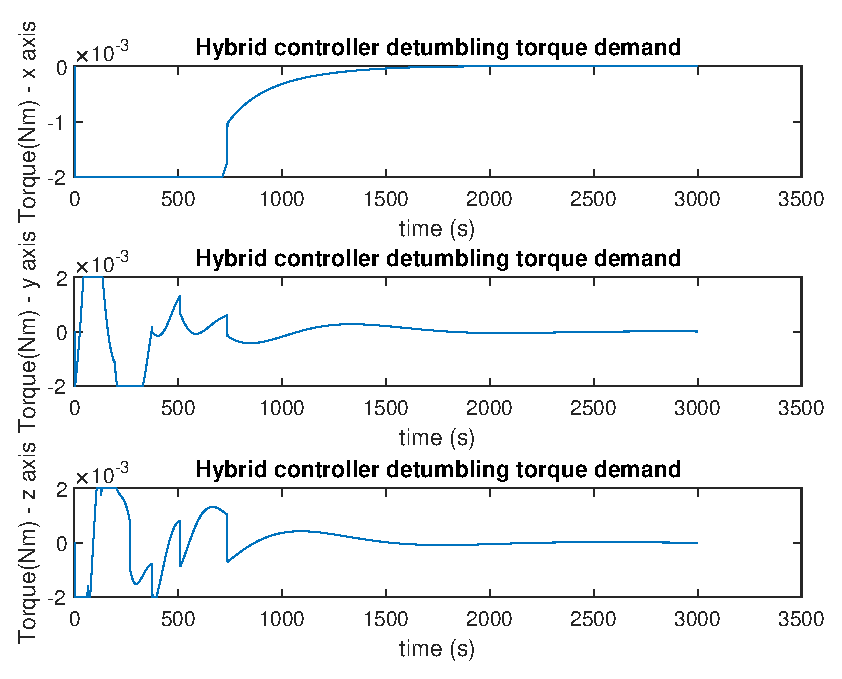
\includegraphics[width=0.7\linewidth]{figures/detumbling}
	\caption{Hybrid controller detumbling torque demand}
	\label{fig:detumbling}
\end{figure}

\begin{figure}[H]
	\centering
	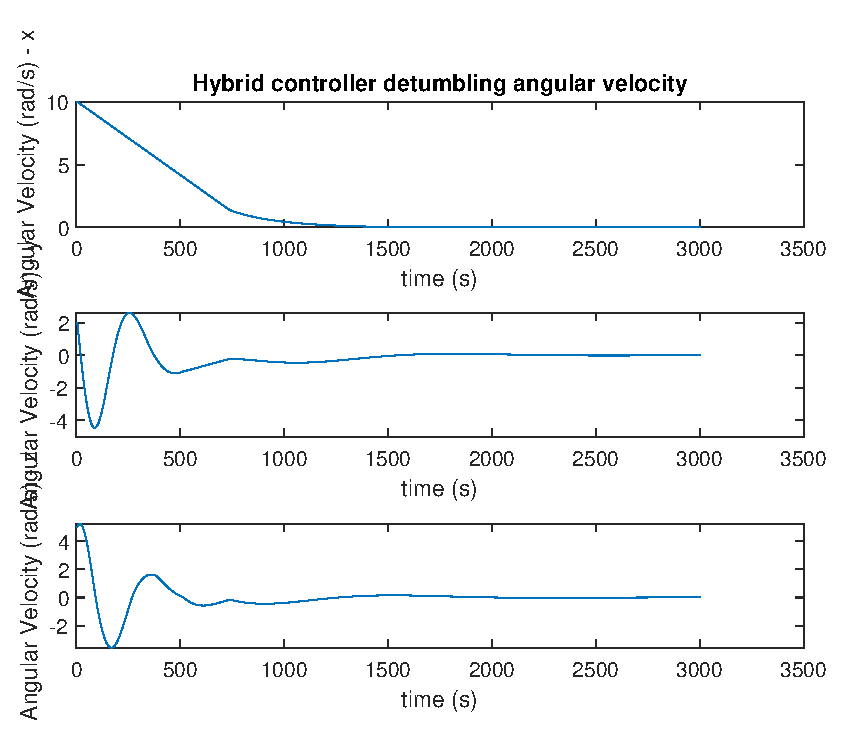
\includegraphics[width=0.7\linewidth]{figures/detumbling3}
	\caption{Hybrid controller detumbling angular velocity}
	\label{fig:omega}
\end{figure}



\input{chapters/OldAttControllers.tex}
